%% LUDUS — CHI submission draft.  Build: see paper/README.md
%% ACM sigconf; review+anonymous for submission.
\documentclass[sigconf,review,anonymous]{acmart}

\usepackage{tikz}
\usetikzlibrary{positioning,arrows.meta,fit,backgrounds,shapes.geometric,calc}
\usepackage{booktabs}
\usepackage{xcolor}
\usepackage{xspace}

%% Placeholder marker for unverified numbers / TODO content. Visible in review.
\newcommand{\PH}[1]{\textcolor{red}{\textbf{[#1]}}}
%% Project name (PLACEHOLDER — "ludus" is Latin for both "game" and "school").
\newcommand{\sys}{\textsc{Ludus}\xspace}

\settopmatter{printacmref=false}
\setcopyright{none}
\acmConference[CHI '26]{ACM CHI Conference on Human Factors in Computing Systems}{2026}{}
\acmISBN{}\acmDOI{}

\begin{document}

\title{\sys: Playable Lessons — A Game-Inspired State-Machine Substrate for
Authoring and Agentically Generating Interactive, Adaptive Educational Experiences}

\author{Anonymous Author(s)}
\affiliation{\institution{Anonymous Institution}\country{}}

\begin{abstract}
Generative AI can draft educational text, but \emph{interactive} learning
experiences---animated explanatory video, adaptive tutorials, responsive
readers---remain hard to author and harder to generate reliably: a single
``make me a lesson'' prompt overflows context, fails opaquely, and produces
artifacts that are neither editable nor adaptive. We present \sys, a substrate
that reframes an interactive lesson as a \emph{playable environment} governed by
a game-style hierarchical state machine and decomposed into atomic, composable
units we call \emph{beats} (grouped into \emph{acts}). The learner is a
``player'': their actions---clicks, answers, free text, and lower-level
\emph{signals} such as gaze or LLM comprehension judgments---are events, and
pedagogy (branching, remediation, pacing) is routing over a shared blackboard.
The same representation does triple duty. (i)~As a \emph{runtime}, it yields
adaptive, multimodal, replayable experiences. (ii)~As a \emph{generation
substrate}, atomic beats let an LLM agent author and verify \emph{one unit
within a small context window}, turning open-ended generation into bounded,
parallel, individually-checkable sub-tasks. (iii)~As a \emph{cross-modal
environment}, it drives both interactive \emph{video} (a continuous per-beat
timeline under a single authoritative clock, with agentic 3D/visual-demo
pipelines) and interactive \emph{reading}, where a knowledge graph parsed from a
book becomes the environment and the reader is the player. We describe the
representation and its design rationale, an agentic generation pipeline, and two
instantiations; we report a technical evaluation of the
decomposition's effect on generation reliability and a user study of authoring
and learning. \PH{Results summary to be filled after studies.}
\end{abstract}

\keywords{interactive learning, generative AI, LLM agents, state machines,
educational video, knowledge graphs, adaptive systems, authoring tools}

\maketitle

%% ---------------------------------------------------------------------------
\begin{figure}[t]
  \centering
  \resizebox{\columnwidth}{!}{% ===========================================================================
% FIG: System architecture — the shared substrate + two instantiations.
% ASCII PREVIEW:
%
%   ┌──────────────────────────────────────────────────────────────┐
%   │  AGENTIC AUTHORING  (LLM agents, one per beat — small context) │
%   └───────────────┬───────────────────────────┬───────────────────┘
%                   │ emit/verify beats          │
%   ┌───────────────▼───────────────┐  ┌─────────▼──────────────────┐
%   │  Interactive VIDEO generation  │  │  Knowledge-GRAPH reader     │
%   │  (beats→timeline, 3D/demos)    │  │  (KG = environment)         │
%   └───────────────┬───────────────┘  └─────────┬──────────────────┘
%                   └─────────────┬───────────────┘
%                  ┌──────────────▼───────────────┐
%                  │   LESSON layer (beats/acts,   │
%                  │   compile flow→transitions)   │
%                  └──────────────┬───────────────┘
%                  ┌──────────────▼───────────────┐
%                  │  GENERIC STATE MACHINE        │
%                  │  (states, routing, blackboard,│
%                  │   open signal channel)        │
%                  └───────────────────────────────┘
%      learner actions ▲  │ render intents / scene snapshots
%                      │  ▼
%                  ┌───────────────────────────────┐
%                  │  RENDERERS (web · video · text)│
%                  └───────────────────────────────┘
% ===========================================================================
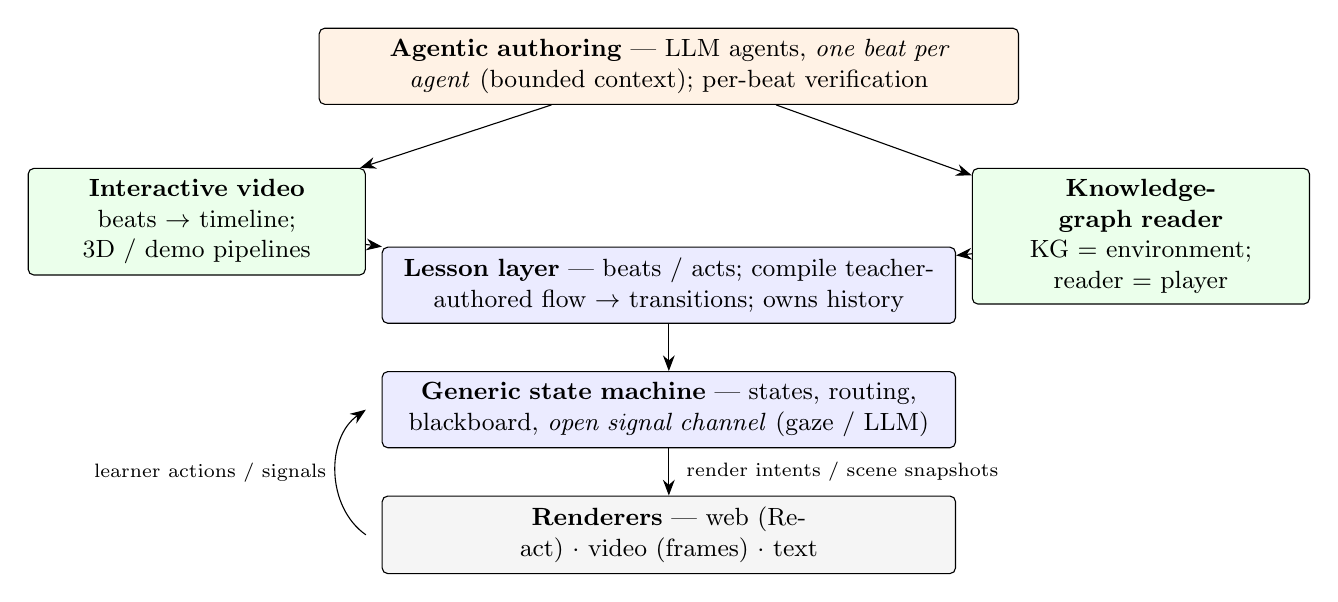
\begin{tikzpicture}[
  font=\small,
  box/.style={draw, rounded corners=2pt, align=center, inner sep=4pt, minimum height=8mm},
  core/.style={box, fill=blue!8},
  app/.style={box, fill=green!8},
  gen/.style={box, fill=orange!10},
  rend/.style={box, fill=gray!8},
  >={Stealth[length=2mm]},
]
\node[gen, text width=86mm] (agents) {\textbf{Agentic authoring} — LLM agents, \emph{one beat per agent} (bounded context); per-beat verification};
\node[app, below left=8mm and -6mm of agents, text width=40mm] (video) {\textbf{Interactive video} \\ beats $\to$ timeline; 3D / demo pipelines};
\node[app, below right=8mm and -6mm of agents, text width=40mm] (reader) {\textbf{Knowledge-graph reader} \\ KG = environment; reader = player};
\node[core, below=18mm of agents, text width=70mm] (lesson) {\textbf{Lesson layer} — beats / acts; compile teacher-authored flow $\to$ transitions; owns history};
\node[core, below=6mm of lesson, text width=70mm] (sm) {\textbf{Generic state machine} — states, routing, blackboard, \emph{open signal channel} (gaze / LLM)};
\node[rend, below=6mm of sm, text width=70mm] (rend) {\textbf{Renderers} — web (React) $\cdot$ video (frames) $\cdot$ text};

\draw[->] (agents) -- (video);
\draw[->] (agents) -- (reader);
\draw[->] (video) -- (lesson);
\draw[->] (reader) -- (lesson);
\draw[->] (lesson) -- (sm);
\draw[->] (sm) -- node[right=1mm, font=\scriptsize]{render intents / scene snapshots} (rend);
\draw[->] ([xshift=-2mm]rend.west) to[bend left=55] node[left, font=\scriptsize]{learner actions / signals} ([xshift=-2mm]sm.west);
\end{tikzpicture}
}
  \caption{\sys{} layers. A generic state machine (states, routing, blackboard,
  open signal channel) carries a lesson layer of \emph{beats/acts}; renderers
  target web, video, and text. The \emph{same} substrate underlies two
  instantiations---interactive video generation and a knowledge-graph
  reader---and is authored by LLM agents one beat at a time.}
  \label{fig:arch}
\end{figure}

%% ---------------------------------------------------------------------------
\section{Introduction}

Decades of research show that interactivity and adaptivity drive learning:
intelligent tutoring systems approach human-tutor effectiveness when they adapt
to the learner~\cite{vanlehn2011relative,anderson1995cognitive}, and
well-designed multimedia reduces extraneous cognitive
load~\cite{mayer2002multimedia,sweller1988cognitive}. Yet the most compelling
interactive explanatory media---animated mathematical videos in the style of
Manim~\cite{manim}, explorable explanations~\cite{victor2011explorable}, and
interactive articles~\cite{hohman2020scrolly}---are painstakingly handcrafted.
Large language models promise to automate this, but applying them naively fails
in three linked ways. First, \textbf{scale}: prompting a model to ``generate a
complete interactive lesson'' exceeds a usable context window, and errors
compound silently across a long generation. Second, \textbf{editability}:
models emit code or markup that is hard to inspect, diff, validate, or hand back
to a teacher. Third, \textbf{adaptivity}: a generated artifact is typically a
fixed script, not an environment that responds to what a particular learner
does, looks at, or misunderstands.

We argue these are symptoms of a missing \emph{representation}. Our key idea is
to borrow from game design~\cite{millington2019ai}: model an interactive lesson
as a \emph{playable environment}---a hierarchical state machine with a shared
``blackboard'' of learner state~\cite{harel1987statecharts}---and decompose it
into atomic, composable \emph{beats}. A beat is the smallest unit of
experience: show an explanation, pose a question, play an animation, probe a
concept. The learner is the \emph{player}; their actions and signals are events;
the teacher (or an agent) authors the \emph{flow} that routes between beats
(Fig.~\ref{fig:player}).

This single representation resolves all three failures at once. It is the
runtime (an event-driven, replayable, adaptive engine); it is the unit of
generation (an agent writes one beat with local context, and the structure
composes the pieces, Fig.~\ref{fig:agentic}); and it is modality-agnostic---the
same beats drive interactive \emph{video} (Fig.~\ref{fig:video}) and interactive
\emph{reading} over a knowledge-graph environment (Fig.~\ref{fig:kg}).

\paragraph{Contributions.}
\begin{enumerate}
\item \textbf{A representation} for interactive learning experiences---a
generic hierarchical state machine with a blackboard and an \emph{open signal
channel}---that is simultaneously human-authorable, agent-authorable,
replayable, and adaptive, with the strict separation of engine, content, and
presentation that makes each independently testable.
\item \textbf{Modular decomposition as the enabler of reliable agentic
generation}: we show that atomic beats let each LLM agent operate within a
bounded context and be verified independently, and we quantify the effect on
generation success, repair, cost, and parallelism versus monolithic generation.
\item \textbf{Two instantiations} on the shared substrate: an agentic
\emph{interactive-video} generator (continuous per-beat timelines under a single
authoritative clock, plus 3D/visual-demo pipelines), and a \emph{knowledge-graph
reader} in which a parsed book becomes the environment and the reader the
player.
\item \textbf{An open signal channel} that makes experiences responsive to
gaze and LLM comprehension judgments \emph{without} engine changes, and remains
auditable and replayable because every adaptive decision is a recorded event.
\end{enumerate}

%% ---------------------------------------------------------------------------
\section{Related Work}

\paragraph{Intelligent tutoring and adaptive learning.} Cognitive
tutors~\cite{anderson1995cognitive} and the broader ITS
literature~\cite{vanlehn2011relative} establish that adaptivity---selecting the
next activity from a model of the learner---is the lever for effectiveness.
\sys{} reuses this insight but treats the \emph{adaptation policy} as data over a
general environment rather than a bespoke tutor, and admits modern signals
(gaze~\cite{dmello2012gaze}, LLM judgments) on a uniform channel.

\paragraph{Explanatory and explorable media.} Manim~\cite{manim},
explorable explanations~\cite{victor2011explorable}, and interactive
articles~\cite{hohman2020scrolly} demonstrate the pedagogical power of animation
and direct manipulation, but are authored by hand. \sys{} aims to retain their
expressive ceiling (a light scene graph and timeline per beat) while making the
artifact a structured, generable, adaptive environment.

\paragraph{Generative AI and LLM agents.} Chain-of-thought
prompting~\cite{wei2022chain} and multi-agent
systems~\cite{park2023generative} improve reliability through decomposition;
retrieval grounds generation in sources~\cite{lewis2020rag}. We contribute a
\emph{domain decomposition}---the beat---that bounds each agent's context and
makes its output independently verifiable against a typed schema.

\paragraph{State machines and game AI.} Harel
statecharts~\cite{harel1987statecharts} give us hierarchy, guards, and a context
blackboard; game AI~\cite{millington2019ai} contributes the
blackboard/environment split and the event-driven loop. We deliberately avoid
behaviour-tree-style continuous re-evaluation: a lesson advances on discrete
learner events, so an event-driven statechart is the better fit.

%% ---------------------------------------------------------------------------
\begin{figure}[t]
  \centering
  \resizebox{\columnwidth}{!}{% ===========================================================================
% FIG: The learner-as-player loop. Content is an environment (a state machine);
% learner actions + signals are events; pedagogy is routing over a blackboard.
% ASCII PREVIEW:
%
%        learner action (click/answer)        gaze / LLM-judgment SIGNALS
%                 │                                     │
%                 ▼                                     ▼
%        ┌───────────────────────────────────────────────────┐
%        │   ENVIRONMENT = statechart   [current beat]         │
%        │   guards read ── BLACKBOARD (score, attempts, vars) │
%        │   routing decides next beat (incl. match: LLM picks │
%        │   among PRE-AUTHORED edges)                         │
%        └───────────────┬───────────────────────────────────┘
%                        │ render intents / scene snapshot
%                        ▼
%                 ┌──────────────┐   every decision is a
%                 │   RENDER      │   RECORDED event  ──► replay / audit
%                 └──────────────┘
% ===========================================================================
\begin{tikzpicture}[
  font=\small, >={Stealth[length=2mm]},
  ev/.style={draw, rounded corners=2pt, fill=orange!10, align=center, inner sep=3pt},
  env/.style={draw, rounded corners=3pt, fill=blue!8, align=center, inner sep=6pt, text width=66mm},
  out/.style={draw, rounded corners=2pt, fill=gray!8, align=center, inner sep=3pt},
]
\node[ev, text width=34mm] (act) {learner action\\(click / answer / free text)};
\node[ev, right=10mm of act, text width=34mm] (sig) {\textbf{signals}\\gaze $\cdot$ LLM judgment};
\node[env, below=10mm of $(act)!0.5!(sig)$] (env) {\textbf{Environment $=$ statechart} \quad[active beat]\\[2pt]
  guards read the \textbf{blackboard} (score, attempts, vars)\\
  routing $\to$ next beat \;(\texttt{match}: a policy picks among \emph{pre-authored} edges)};
\node[out, below=9mm of env, text width=40mm] (render) {\textbf{render} intents / scene snapshot};
\node[out, right=12mm of render, text width=38mm, fill=green!8] (log) {every decision is a\\\textbf{recorded event}\\$\Rightarrow$ replay \& audit};

\draw[->] (act) -- (env);
\draw[->] (sig) -- (env);
\draw[->] (env) -- (render);
\draw[->] (env.east) -- (log.north);
\draw[->] (render.west) to[bend left=45] node[left,font=\scriptsize]{loop} (env.west);
\end{tikzpicture}
}
  \caption{The learner-as-player loop. The content \emph{is} an environment;
  learner actions and signals are events; routing over the blackboard selects
  the next beat. Adaptive policies (incl. an LLM) select among \emph{pre-authored}
  edges via \texttt{match}, never inventing jumps. Every decision is a recorded
  event, so sessions replay and audit.}
  \label{fig:player}
\end{figure}

%% ---------------------------------------------------------------------------
\section{The \sys{} Representation}
\label{sec:rep}

\subsection{Environment, blackboard, signals}
A lesson is a hierarchical state machine $\langle S, s_0, T\rangle$ over a
context $C$ (the blackboard: score, attempts, teacher variables, and a complete
event history). Transitions carry \emph{guards} (pure predicates over $C$ and the
event) and \emph{actions} (declarative context patches plus \emph{effects}).
Crucially, the engine is \emph{generic}: it knows nothing of lessons, beats, or
rendering---a property we verify with a non-lesson ``turnstile'' machine that
exercises the engine with a toy context. This keeps the core small, testable,
and reusable.

The \textbf{open signal channel} is the design move that admits adaptivity
without special-casing. Events are an open type: alongside
\texttt{answer} or \texttt{next}, the engine accepts \texttt{signal.confused} or
\texttt{llm.misconception:$x$}. Such signals are produced by external
adapters---a gaze tracker, an LLM judge---and aggregated into \emph{semantic}
events before entering the machine, where guards read them and routes act on
them. Because the engine is a pure reducer, every event (including every
adaptive verdict) is recorded; a session is reconstructable by replay, and the
log explains \emph{why} each adaptive route fired.

\subsection{Beats and acts; the teacher owns the flow}
A \emph{beat} is a parameterized, reusable building block compiled into a small
sub-machine: \textsc{Explain}, \textsc{Mcq}, \textsc{Branch}, \textsc{Animate}.
Beats group into \emph{acts}. A central principle---learned during design---is
that \textbf{the teacher (or agent) owns the flow}: branching is authored
\emph{data}, not an engine feature and not a fixed policy. A compiler lowers
authored flow (a linear ``spine'' plus detours such as remediation) into
explicit transitions; \texttt{mcq$\to$remediate} is one convenience, not a
built-in. Adaptive policies, including LLMs, are therefore \emph{selectors over
the teacher's graph} (via a \texttt{match} route that maps an event payload to a
pre-authored target), never authors of arbitrary jumps. This keeps generated and
adapted lessons auditable and safe.

\subsection{Separation of engine, content, and presentation}
Content is emitted as typed, presentation-free \emph{render intents}
(text/visual/mcq/scene) tagged with named \emph{slots}; a \emph{template} maps
slots to regions and content kinds to components, and supplies theme tokens. The
lesson never names a pixel; swapping the template re-skins or re-targets the
same lesson---including, as \S\ref{sec:video} shows, to video. Effects (timers,
network, TTS, LLM calls) are run by a shell with structured cancellation, so the
reducer stays pure and nondeterminism re-enters only as recorded events.

%% ---------------------------------------------------------------------------
\section{Modular Generation: Beats as Agentic Decomposition}
\label{sec:agentic}

\begin{figure}[t]
  \centering
  \resizebox{\columnwidth}{!}{% ===========================================================================
% FIG: Modular decomposition enables small-context agentic generation.
% A monolithic "generate the whole lesson" prompt overflows context and fails
% opaquely; beats/acts let each agent author ONE atomic unit, verified locally,
% composed by the structure.
% ASCII PREVIEW:
%
%   topic + objectives
%        │
%        ▼  (planner: outline = ordered beats/acts)
%   ┌──────────────────────────────────────────────┐
%   │  act 1        act 2              act 3         │
%   │  [b1][b2]     [b3][b4][b5]       [b6][b7]      │
%   └───┬───┬────────┬───┬───┬──────────┬───┬───────┘
%       ▼   ▼        ▼   ▼   ▼          ▼   ▼     one AGENT per beat
%      🤖  🤖       🤖  🤖  🤖         🤖  🤖    (small context window)
%       │   │        │   │   │          │   │
%       └───┴───►  per-beat VALIDATE / repair  ◄──┴───┘
%                          │
%                          ▼
%                  compile → runnable lesson (statechart)
% ===========================================================================
\begin{tikzpicture}[
  font=\small, >={Stealth[length=2mm]},
  beat/.style={draw, rounded corners=1.5pt, fill=blue!8, minimum width=7mm, minimum height=6mm, inner sep=1pt, font=\scriptsize},
  agent/.style={draw, circle, fill=orange!12, inner sep=1pt, minimum size=7mm, font=\tiny},
  lbl/.style={align=center, font=\scriptsize},
  stage/.style={align=center, inner sep=3pt},
]
\node[stage] (top) {\textbf{topic + objectives}};
\node[stage, below=5mm of top, draw, rounded corners=2pt, fill=gray!8, text width=70mm]
  (plan) {\textbf{planner agent} $\to$ outline as ordered \emph{acts} of \emph{beats}};

% beats row
\node[beat, below=8mm of plan.west, anchor=west, xshift=2mm] (b1) {b1};
\foreach \i/\p in {2/b1,3/b2,4/b3,5/b4,6/b5,7/b6}{
  \node[beat, right=2.2mm of b\p] (b\i) {b\i};
}
\node[lbl, right=4mm of b7] {\emph{acts group beats}};

% agents under beats
\foreach \i in {1,...,7}{
  \node[agent, below=7mm of b\i] (a\i) {LLM};
  \draw[->] (b\i) -- (a\i);
}
\draw[->] (plan.south) -- ($(b4.north)+(0,2mm)$);

\node[stage, below=8mm of a4, draw, rounded corners=2pt, fill=green!8, text width=66mm]
  (val) {\textbf{per-beat validate / repair} (bounded context; parallel)};
\foreach \i in {1,...,7}{ \draw[->] (a\i) -- (val.north); }

\node[stage, below=5mm of val, draw, rounded corners=2pt, fill=blue!12, text width=58mm]
  (comp) {\textbf{compile} $\to$ runnable lesson (statechart)};
\draw[->] (val) -- (comp);
\end{tikzpicture}
}
  \caption{Generation as composition. A planner emits an outline of acts/beats;
  one agent authors each beat within a \emph{bounded} context; each beat is
  validated/repaired against a typed schema, in parallel; the compiler assembles
  a runnable statechart. Contrast with a monolithic prompt that must hold the
  whole lesson at once.}
  \label{fig:agentic}
\end{figure}

The atomicity of beats is what makes agentic generation reliable. Our pipeline
(Fig.~\ref{fig:agentic}) mirrors the two-stage planning that proved effective in
prior systems: a \emph{planner} reasons about pedagogy and emits an outline as an
ordered set of acts/beats with declared learning objectives and a visual
contract; then \emph{worker} agents each author a single beat---its content,
its choices, its storyboard---seeing only local context (the objective, the
neighbouring beats' summaries, the shared style). Each beat is independently
\textbf{validated} against a typed schema and, on failure, \textbf{repaired}
with the validator's error fed back, never blocking its siblings. A
\emph{deterministic} compiler (no LLM) assembles the validated beats into a
statechart, and a structural validator rejects dangling targets, unknown beats,
unreachable nodes, and flows with no terminal---turning a bad generation into a
precise message rather than a runtime failure.

Three properties follow directly. \emph{Bounded context}: each agent's prompt
is $O(\text{one beat})$, independent of lesson length. \emph{Parallelism}: beats
are generated and verified concurrently. \emph{Local verifiability}: a beat is a
self-contained, typed, replayable unit, so correctness is checked per unit
rather than over an entire artifact. \S\ref{sec:tech} quantifies these.

\subsection{Agentic 3D and visual-demo generation}
Visual beats require figures, animations, and occasionally 3D scenes. Because a
beat declares a \emph{visual contract} (the methods/props its animation needs),
a specialized visual agent fills only that contract, and a \emph{sighted}
revision step can inspect a rendered preview and self-correct. Crucially,
animations are \textbf{declarative data} (a storyboard of scene-graph primitives
and tweens), not executed code; this preserves replay, enables validation, and
avoids the security and reliability hazards of generating and \texttt{eval}-ing
code.

%% ---------------------------------------------------------------------------
\section{Interactive Video Generation}
\label{sec:video}

\begin{figure}[t]
  \centering
  \resizebox{\columnwidth}{!}{% ===========================================================================
% FIG: The discrete+continuous video model. The state machine sequences beats
% (discrete); each beat carries a Storyboard timeline (continuous); ONE clock
% (beat time t) drives a pure sampleAt(); the same function feeds interactive
% playback AND offline frame export. Audio/subtitles are slaved to t (no drift).
% ASCII PREVIEW:
%
%   SM (discrete):   [intro] ─► [explain*] ─► [quiz] ─► ...      *timed beat
%                                  │  beat time t ∈ [0,dur]
%                                  ▼
%             Storyboard ── sampleAt(t) ──► SceneSnapshot ─┬─► PLAYER (rAF loop)
%               tweens, cues                               └─► EXPORT (per frame→mp4)
%                                  │
%               audio + word-level subtitles  ── slaved to t (one clock)
%             at t=dur ► emit beat.done ► SM advances
% ===========================================================================
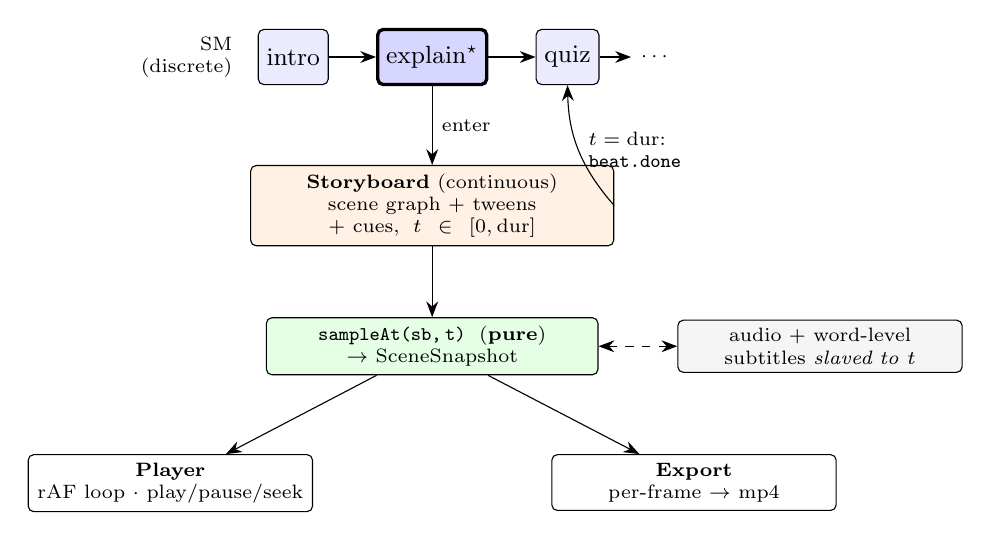
\begin{tikzpicture}[
  font=\small, >={Stealth[length=2mm]},
  beat/.style={draw, rounded corners=2pt, fill=blue!8, minimum height=7mm, inner sep=3pt, font=\small},
  tbeat/.style={beat, fill=blue!16, very thick},
  proc/.style={draw, rounded corners=2pt, align=center, inner sep=3pt, font=\scriptsize},
]
% discrete SM row
\node[beat] (b0) {intro};
\node[tbeat, right=6mm of b0] (b1) {explain$^\star$};
\node[beat, right=6mm of b1] (b2) {quiz};
\node[right=4mm of b2, font=\scriptsize] (dots) {$\cdots$};
\draw[->] (b0) -- (b1); \draw[->] (b1) -- (b2); \draw[->] (b2) -- (dots);
\node[left=2mm of b0, font=\scriptsize, align=right] {SM\\(discrete)};

% timeline of the timed beat
\node[proc, fill=orange!10, below=10mm of b1, text width=44mm]
  (sb) {\textbf{Storyboard} (continuous)\\ scene graph + tweens + cues,\; $t\in[0,\mathrm{dur}]$};
\draw[->] (b1) -- node[right,font=\scriptsize]{enter} (sb);

\node[proc, fill=green!10, below=9mm of sb, text width=40mm]
  (sample) {\texttt{sampleAt(sb,\,t)} \;(\textbf{pure})\\$\to$ SceneSnapshot};
\draw[->] (sb) -- (sample);

\node[proc, below left=10mm and -6mm of sample, text width=34mm] (play) {\textbf{Player}\\rAF loop $\cdot$ play/pause/seek};
\node[proc, below right=10mm and -6mm of sample, text width=34mm] (exp) {\textbf{Export}\\per-frame $\to$ mp4};
\draw[->] (sample) -- (play);
\draw[->] (sample) -- (exp);

\node[proc, fill=gray!8, right=10mm of sample, text width=34mm]
  (audio) {audio + word-level\\subtitles \emph{slaved to }$t$};
\draw[<->, dashed] (sample) -- (audio);

% beat.done back to SM
\draw[->] (sb.east) to[bend left=20] node[right,font=\scriptsize,align=left]{$t=\mathrm{dur}$:\\\texttt{beat.done}} (b2.south);
\end{tikzpicture}
}
  \caption{Reconciling discrete interaction with continuous animation. The state
  machine sequences beats (discrete); each timed beat carries a \emph{storyboard}
  (continuous); a single authoritative clock $t$ drives a \emph{pure}
  \texttt{sampleAt}. The same function feeds interactive playback and offline
  frame export; audio and word-level subtitles are slaved to $t$. At $t=\text{dur}$
  the clock emits \texttt{beat.done} and the machine advances.}
  \label{fig:video}
\end{figure}

Interactive video is where the discrete/continuous tension is sharpest: a lesson
advances on discrete events, but animation is continuous in time. \sys{}
reconciles them with one rule (Fig.~\ref{fig:video}): \textbf{the state machine
sequences beats (discrete); each beat carries a timeline (continuous); a single
authoritative clock---beat time $t$---drives everything.} The linchpin is a pure
function $\texttt{sampleAt}(\textit{storyboard}, t)\!\to\!\textit{snapshot}$,
shared by three consumers: an interactive \emph{player} samples it in an
animation loop; \emph{seek/scrub} samples at an arbitrary $t$ (replaying events
to reach the beat); and \emph{offline export} samples at each frame time to emit
video. Audio (with word-level subtitles from TTS) is \emph{slaved} to $t$ rather
than run on its own clock, eliminating the multi-clock drift that plagues
hand-built systems. To the engine, a 30-second animated beat is identical to an
instant one---it simply receives a \texttt{beat.done} event at the timeline's
end---so no engine change is required to gain video.

Both interactive playback and file export thus derive from the same storyboard
and the same sampler, and an animated beat remains an ordinary, interactive
beat: a question can interrupt a video mid-timeline via a \emph{gate} cue, and
adaptivity (\S\ref{sec:rep}) applies unchanged.

%% ---------------------------------------------------------------------------
\section{Knowledge-Graph Environments for Interactive Reading}
\label{sec:kg}

\begin{figure}[t]
  \centering
  \resizebox{\columnwidth}{!}{% ===========================================================================
% FIG: Knowledge-graph-as-environment for interactive reading. A book is parsed
% into a concept KG; the KG becomes the state-machine environment; the reader is
% the player. Reading position + comprehension signals drive routing to the next
% concept / explanation / probe — the SAME substrate as interactive video.
% ASCII PREVIEW:
%
%    BOOK / PDF ──parse──►  KNOWLEDGE GRAPH (concepts, prerequisites)
%                              (o)forces──►(o)energy──►(o)work
%                                 │            ▲
%                                 ▼            │ prereq
%                              (o)vectors ─────┘
%                              │  mapped to a statechart ENVIRONMENT
%                              ▼
%    READER = player ──► position + comprehension signals (gaze/Q&A/LLM)
%                              ▼
%                  routing ► next concept · just-in-time explanation · probe
%                              ▼
%                   chatbot + PDF, co-driven by the same engine
% ===========================================================================
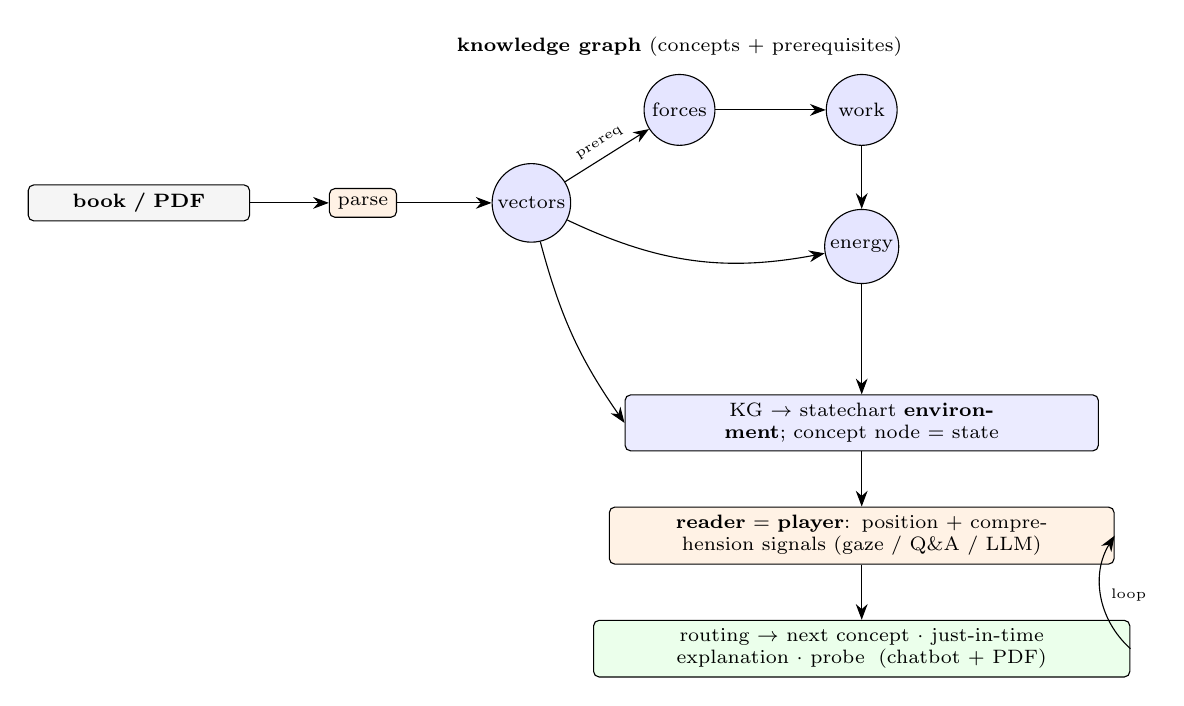
\begin{tikzpicture}[
  font=\small, >={Stealth[length=2mm]},
  c/.style={draw, circle, fill=blue!10, inner sep=1.5pt, minimum size=9mm, font=\scriptsize, align=center},
  box/.style={draw, rounded corners=2pt, align=center, inner sep=3pt, font=\scriptsize},
]
\node[box, fill=gray!8, text width=26mm] (book) {\textbf{book / PDF}};
\node[box, right=10mm of book, fill=orange!10] (parse) {parse};
\draw[->] (book) -- (parse);

% KG
\node[c, right=12mm of parse] (vec) {vectors};
\node[c, above right=5mm and 12mm of vec] (force) {forces};
\node[c, right=14mm of force] (work) {work};
\node[c, below=8mm of work] (energy) {energy};
\draw[->] (parse) -- (vec);
\draw[->] (vec) -- node[above,font=\tiny,sloped]{prereq} (force);
\draw[->] (force) -- node[above,font=\tiny]{} (work);
\draw[->] (work) -- (energy);
\draw[->] (vec) to[bend right=18] (energy);
\node[above=1mm of force, font=\scriptsize] {\textbf{knowledge graph} (concepts + prerequisites)};

% mapping to environment
\node[box, fill=blue!8, below=14mm of energy, text width=58mm]
  (env) {KG $\to$ statechart \textbf{environment}; concept node $=$ state};
\draw[->] (energy) -- (env);
\draw[->] (vec) to[bend right=10] (env.west);

\node[box, fill=orange!10, below=7mm of env, text width=62mm]
  (sig) {\textbf{reader $=$ player}: position $+$ comprehension signals (gaze / Q\&A / LLM)};
\draw[->] (env) -- (sig);
\node[box, fill=green!8, below=7mm of sig, text width=66mm]
  (out) {routing $\to$ next concept $\cdot$ just-in-time explanation $\cdot$ probe \;(chatbot $+$ PDF)};
\draw[->] (sig) -- (out);
\draw[->] (out.east) to[bend left=40] node[right,font=\tiny]{loop} (sig.east);
\end{tikzpicture}
}
  \caption{A companion instantiation. A book/PDF is parsed into a concept
  knowledge graph (concepts + prerequisites); the graph becomes the
  state-machine environment and the reader becomes the player. Reading position
  and comprehension signals route to the next concept, a just-in-time
  explanation, or a probe---surfaced as a chatbot alongside the PDF.}
  \label{fig:kg}
\end{figure}

The same substrate supports a second, complementary experience
(Fig.~\ref{fig:kg}). A book is parsed into a \emph{knowledge graph} of concepts
and prerequisite relations; the graph is mapped to the state-machine
environment, with each concept a state. The reader is the player: reading
position and comprehension signals (questions asked, gaze, LLM assessment of a
free-text answer) become events that route to the next concept, trigger a
just-in-time explanation, or pose a probe---presented as a chatbot beside the
document. Where the video instantiation emphasizes continuous time, the reader
emphasizes non-linear navigation of a concept graph; both are flows over the
same engine, authored and adapted by the same machinery. \PH{Reader system
details from collaborator to be expanded.}

%% ---------------------------------------------------------------------------
\section{Implementation}
\label{sec:impl}

\sys{} is implemented in TypeScript as a set of layered packages with a strict
one-way dependency rule, enforced structurally: a generic \texttt{state\_machine}
(no knowledge of lessons or rendering), a \texttt{render\_contract} of typed
intents, a \texttt{lesson} layer (beats, the flow compiler/validator, and a
session shell that owns history and runs effects with cancellation), a
\texttt{timeline} package (scene graph $+$ storyboards $+$ the pure
\texttt{sampleAt}), and web/video renderers. The engine's genericity is verified
by driving an unrelated turnstile machine through it. The interpreter is a pure
reducer; sessions support $O(1)$ snapshot/restore and $O(n)$ replay from the
event log. \PH{Add LoC, package list, and links to the open-source release.}

%% ---------------------------------------------------------------------------
\section{Technical Evaluation}
\label{sec:tech}

We evaluate the central architectural claim---that beat-level decomposition
makes agentic generation more reliable than monolithic generation---with a
controlled comparison. \emph{This section states the protocol; numbers are
placeholders pending runs.}

\paragraph{Conditions.} (i)~\textsc{Monolithic}: one prompt generates an entire
lesson. (ii)~\textsc{Decomposed} (\sys): planner $+$ per-beat agents $+$ per-beat
validate/repair. Same base model, matched token budgets, $N=\PH{N}$ topics
across $\PH{k}$ subjects.

\paragraph{Metrics.}
\begin{itemize}
\item \textbf{Context per call} (tokens): max and mean prompt size.
\item \textbf{Validity}: fraction compiling without structural errors
(\S\ref{sec:agentic}); mean repair rounds to validity.
\item \textbf{Pedagogical quality}: expert rubric (objective coverage,
scaffolding, correctness) on a 1--5 scale, blind to condition.
\item \textbf{Cost \& latency}: tokens and wall-clock, with and without
beat-level parallelism.
\item \textbf{Editability}: number of localized edits to fix a seeded fault
without regressions.
\end{itemize}

\paragraph{Hypotheses.} H1: \textsc{Decomposed} has dramatically lower max
context per call (by construction, $O(\text{beat})$ vs $O(\text{lesson})$). H2:
\textsc{Decomposed} achieves higher first-pass validity and fewer global
failures. H3: parallel beat generation reduces wall-clock at comparable or lower
total cost. H4: faults are repaired with more localized edits.
\PH{Insert Table~with results: context (max/mean), validity \%, repair rounds,
rubric mean$\pm$sd, tokens, latency.}

%% ---------------------------------------------------------------------------
\section{User Study}
\label{sec:study}

We complement the technical evaluation with two small studies. \emph{Protocols
below; results pending IRB and runs.}

\paragraph{Study A --- Authoring (within-subjects, $n=\PH{n_A}$ educators).}
Participants author a short interactive lesson (a)~with a baseline
slides/video tool and (b)~with \sys{} (agent-assisted, editing beats). Measures:
time to a working lesson, edits accepted/rejected, SUS, NASA-TLX, and a
semi-structured interview on control and trust in agent-authored content.
Hypothesis: \sys{} reduces authoring effort while \emph{increasing} perceived
control, because edits are localized to inspectable beats.

\paragraph{Study B --- Learning \& adaptivity (between-subjects,
$n=\PH{n_B}$ learners).} Conditions: \textsc{Static} (linear video/reading) vs
\textsc{Adaptive} (\sys{} with the open signal channel: branch on quiz outcome;
optional gaze-driven re-explanation). Measures: post-test learning gain,
engagement, self-report, and---in the adaptive arm---an audit of which signals
triggered which routes (enabled by the event log). Hypothesis: adaptivity
improves gain and engagement, and the event-log audit lets us attribute gains to
specific adaptive decisions.

\PH{Insert results, figures (learning-gain bars, TLX, SUS), and qualitative
themes.}

%% ---------------------------------------------------------------------------
\section{Discussion and Limitations}

\sys{} positions adaptivity, generation, and multimodality as facets of one
representation, which we believe is the paper's conceptual core. Several
limitations are worth stating. The current interpreter implements a \emph{flat}
subset of the hierarchical model (events resolve at the top level; deep bubbling
is specified but not yet implemented), which constrains how richly a single beat
can nest sub-interactions. Adaptive policies select among pre-authored
edges---safe and auditable, but it forecloses genuinely emergent paths; whether
that ceiling matters pedagogically is an empirical question. TTS and offline
export add real engineering surface (we mitigate multi-clock drift by a single
authoritative clock, but audio synthesis quality and caching remain practical
concerns). Finally, agentic generation inherits LLM failure modes; our per-beat
validation bounds, but does not eliminate, incorrect content---hence the human
edit loop and the editability metric.

%% ---------------------------------------------------------------------------
\section{Conclusion}

We presented \sys, a game-inspired state-machine substrate that treats an
interactive lesson as a playable environment of atomic beats. The representation
is at once a runtime for adaptive, replayable, multimodal experiences and the
unit of reliable agentic generation, and it spans interactive video and
knowledge-graph reading. By making the learner a player, the teacher the author
of the flow, and the beat the atom of both interaction and generation, \sys{}
offers a path to educational experiences that are generated at scale yet remain
adaptive, auditable, and editable.

\bibliographystyle{ACM-Reference-Format}
\bibliography{refs}

\end{document}
